\documentclass{standalone}
\usepackage{tikz}
\usepackage{pgfplots}
\pgfplotsset{width=32cm,height=18cm,compat=1.3}
\pgfplotsset{every tick label/.append style={font=\Huge}}
\usepackage{filecontents}

\usetikzlibrary{patterns}

\definecolor{citrine}{rgb}{0.89, 0.82, 0.04}

\begin{document}
	\centering
		\vspace{1.5em}
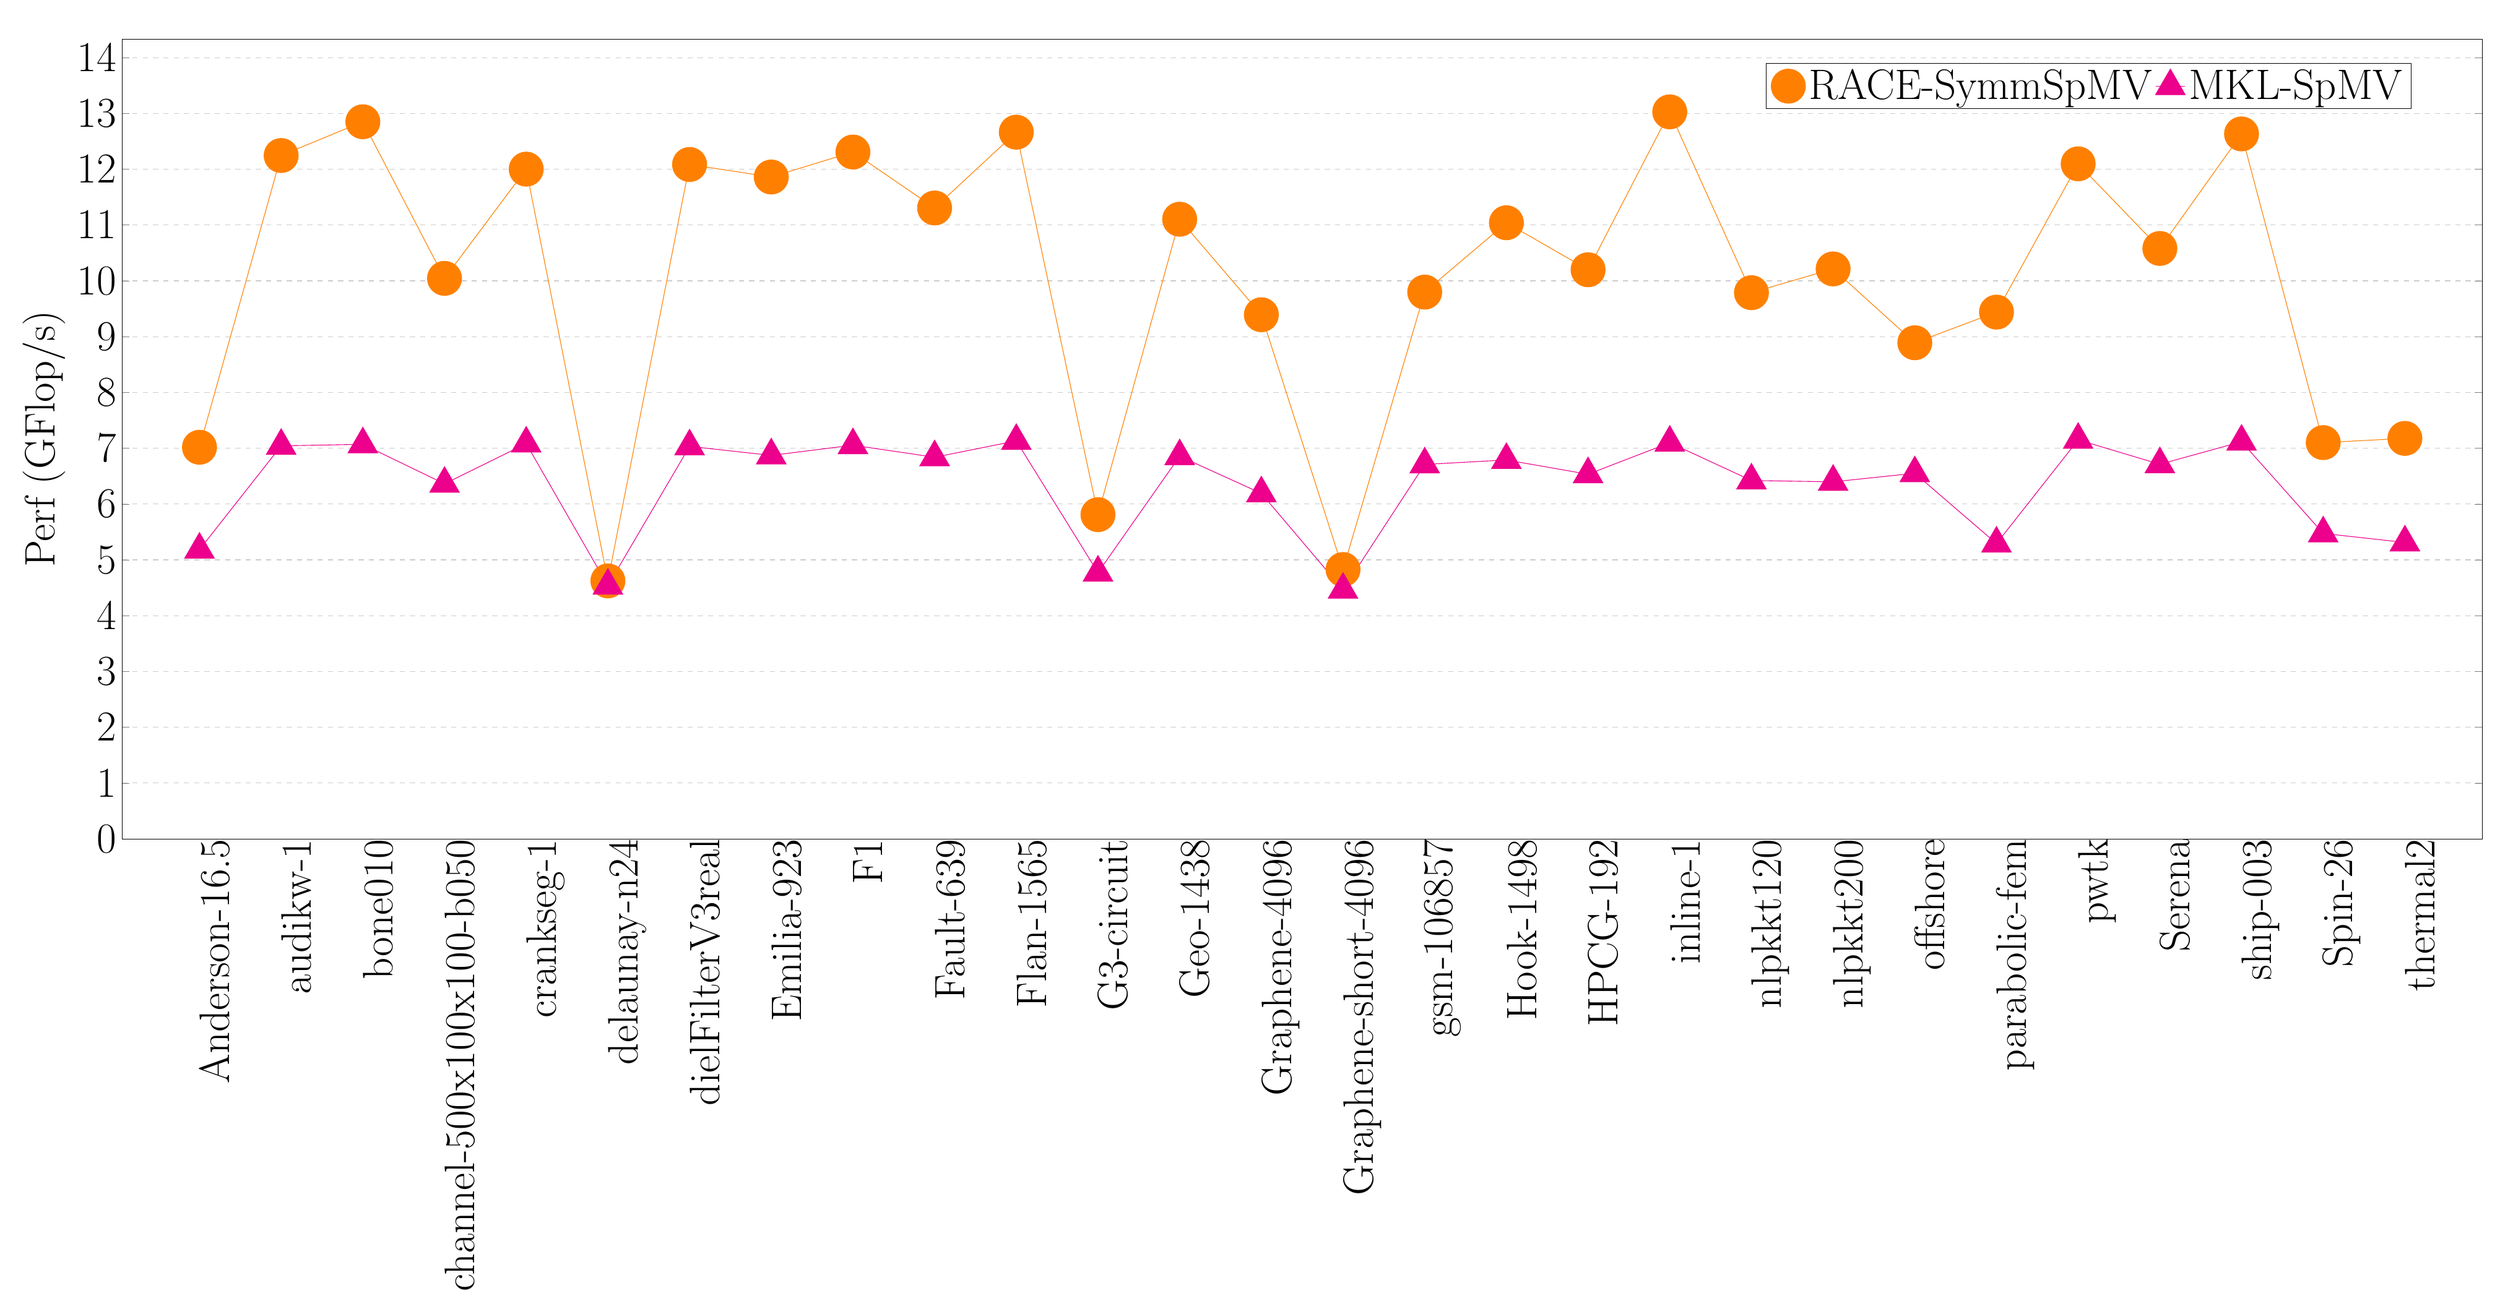
\begin{tikzpicture}
		%	\node at (13.25,15) {\LARGE{}};
			\begin{axis}[
		%	xmin=0.25, xmax=7.25,
			ymin=0, %ymax=3.25,
			xtick={1, 2, 3, 4, 5, 6, 7, 8, 9, 10, 11, 12, 13, 14, 15, 16, 17, 18, 19, 20, 21, 22, 23, 24, 25, 26, 27, 28},
		%	ytick={0,0.5,1,1.5,2,2.5,3},
			xticklabels={Anderson-16.5, audikw-1, bone010, channel-500x100x100-b050, crankseg-1, delaunay-n24, dielFilterV3real, Emilia-923, F1, Fault-639, Flan-1565, G3-circuit, Geo-1438, Graphene-4096, Graphene-short-4096, gsm-106857, Hook-1498, HPCG-192, inline-1, nlpkkt120, nlpkkt200, offshore, parabolic-fem, pwtk, Serena, ship-003, Spin-26, thermal2},
			width  = 50cm,
			height = 18cm,
			major x tick style = transparent,
			%	minor ytick={1, 5, 10, 15, 20, 25, 30 ,35,40},
			grid = minor,	
			%add_bar_commands
			ymajorgrids = true,
			grid style={dashed, gray!40},
			ylabel = {\Huge{Perf (GFlop/s)}},
		%	symbolic x coords={Graphene-2048-2048, Graphene-4096-4096, Spin-24-24-24},
			x tick label style={rotate=90, anchor=north east, inner sep=0mm, font={\Huge}},
			tick label style={font={\Huge}},
			scaled y ticks = false,
			enlarge x limits=0.035,
			legend cell align=left,
			legend style={font=\Huge},
			legend columns=-1,
			legend style={
				%at={(1,1.05)},
				%anchor=south east,
				%column sep=1ex,
				legend pos=north east
			},
			%spl_legend_code
			title= {\Huge\scalebox{1.5}{{}}}
			]

\addplot[mark=*, mark size=10pt, mark options={orange}, draw=orange ] plot coordinates{(1,7.017762) (2,12.245165) (3,12.850634) (4,10.044041) (5,12.001241) (6,4.623104) (7,12.084667) (8,11.860212) (9,12.308086) (10,11.305451) (11,12.663604) (12,5.809891) (13,11.103660) (14,9.392370) (15,4.827286) (16,9.797964) (17,11.040916) (18,10.198226) (19,13.027954) (20,9.787395) (21,10.213585) (22,8.890258) (23,9.439195) (24,12.096590) (25,10.580104) (26,12.632607) (27,7.101122) (28,7.176575)};
\addplot[mark=triangle*, mark size=10pt, mark options={magenta}, draw=magenta ] plot coordinates{(1,5.182545) (2,7.043145) (3,7.070277) (4,6.362534) (5,7.083106) (6,4.537544) (7,7.033526) (8,6.871915) (9,7.054848) (10,6.838865) (11,7.131561) (12,4.770986) (13,6.856778) (14,6.191554) (15,4.464146) (16,6.709915) (17,6.789662) (18,6.534070) (19,7.099324) (20,6.421885) (21,6.398243) (22,6.551354) (23,5.291437) (24,7.150255) (25,6.712824) (26,7.117153) (27,5.473422) (28,5.311964)};
	%addplot cmd

	\legend{RACE-SymmSpMV, MKL-SpMV}

	\end{axis}			
\end{tikzpicture}

\end{document}

